% !TEX root = template.tex

\section{Taxonomy}

To explore the taxonomic distribution of proteins within our family, we systematically collected and analyzed lineage data for the $83$ sequences identified. Using protein identifiers from PSI-BLAST and HMM-SEARCH, we queried the UniProt API~\cite{uniprot_api} to retrieve the complete taxonomic lineage for each protein, capturing their hierarchical classification from the broadest domain (\textit{Eukaryota}) to the most specific organism. The taxonomic tree was generated using the ETE Toolkit~\cite{ete_toolkit} and visualized in the Newick tree format~\cite{newick_format}. Node sizes in the phylogenetic tree were adjusted to reflect the relative abundance of each taxonomic entity, with larger nodes indicating higher representation in the protein family. Fig.~\ref{fig:phylo-tree} illustrates the resulting phylogenetic tree, highlighting the distribution of proteins across various taxonomic groups. To further analyze taxonomic diversity, we processed the collected lineage data to calculate frequency counts at each taxonomic level. By traversing the hierarchical taxonomy, we generated a nested dictionary that revealed the occurrence patterns of each taxonomic node across the dataset. These clustering patterns underscore the evolutionary pressures maintaining the functionality of this domain across diverse taxa, providing insights into its conserved biological roles.

\begin{figure*}[h!]
    \centering
    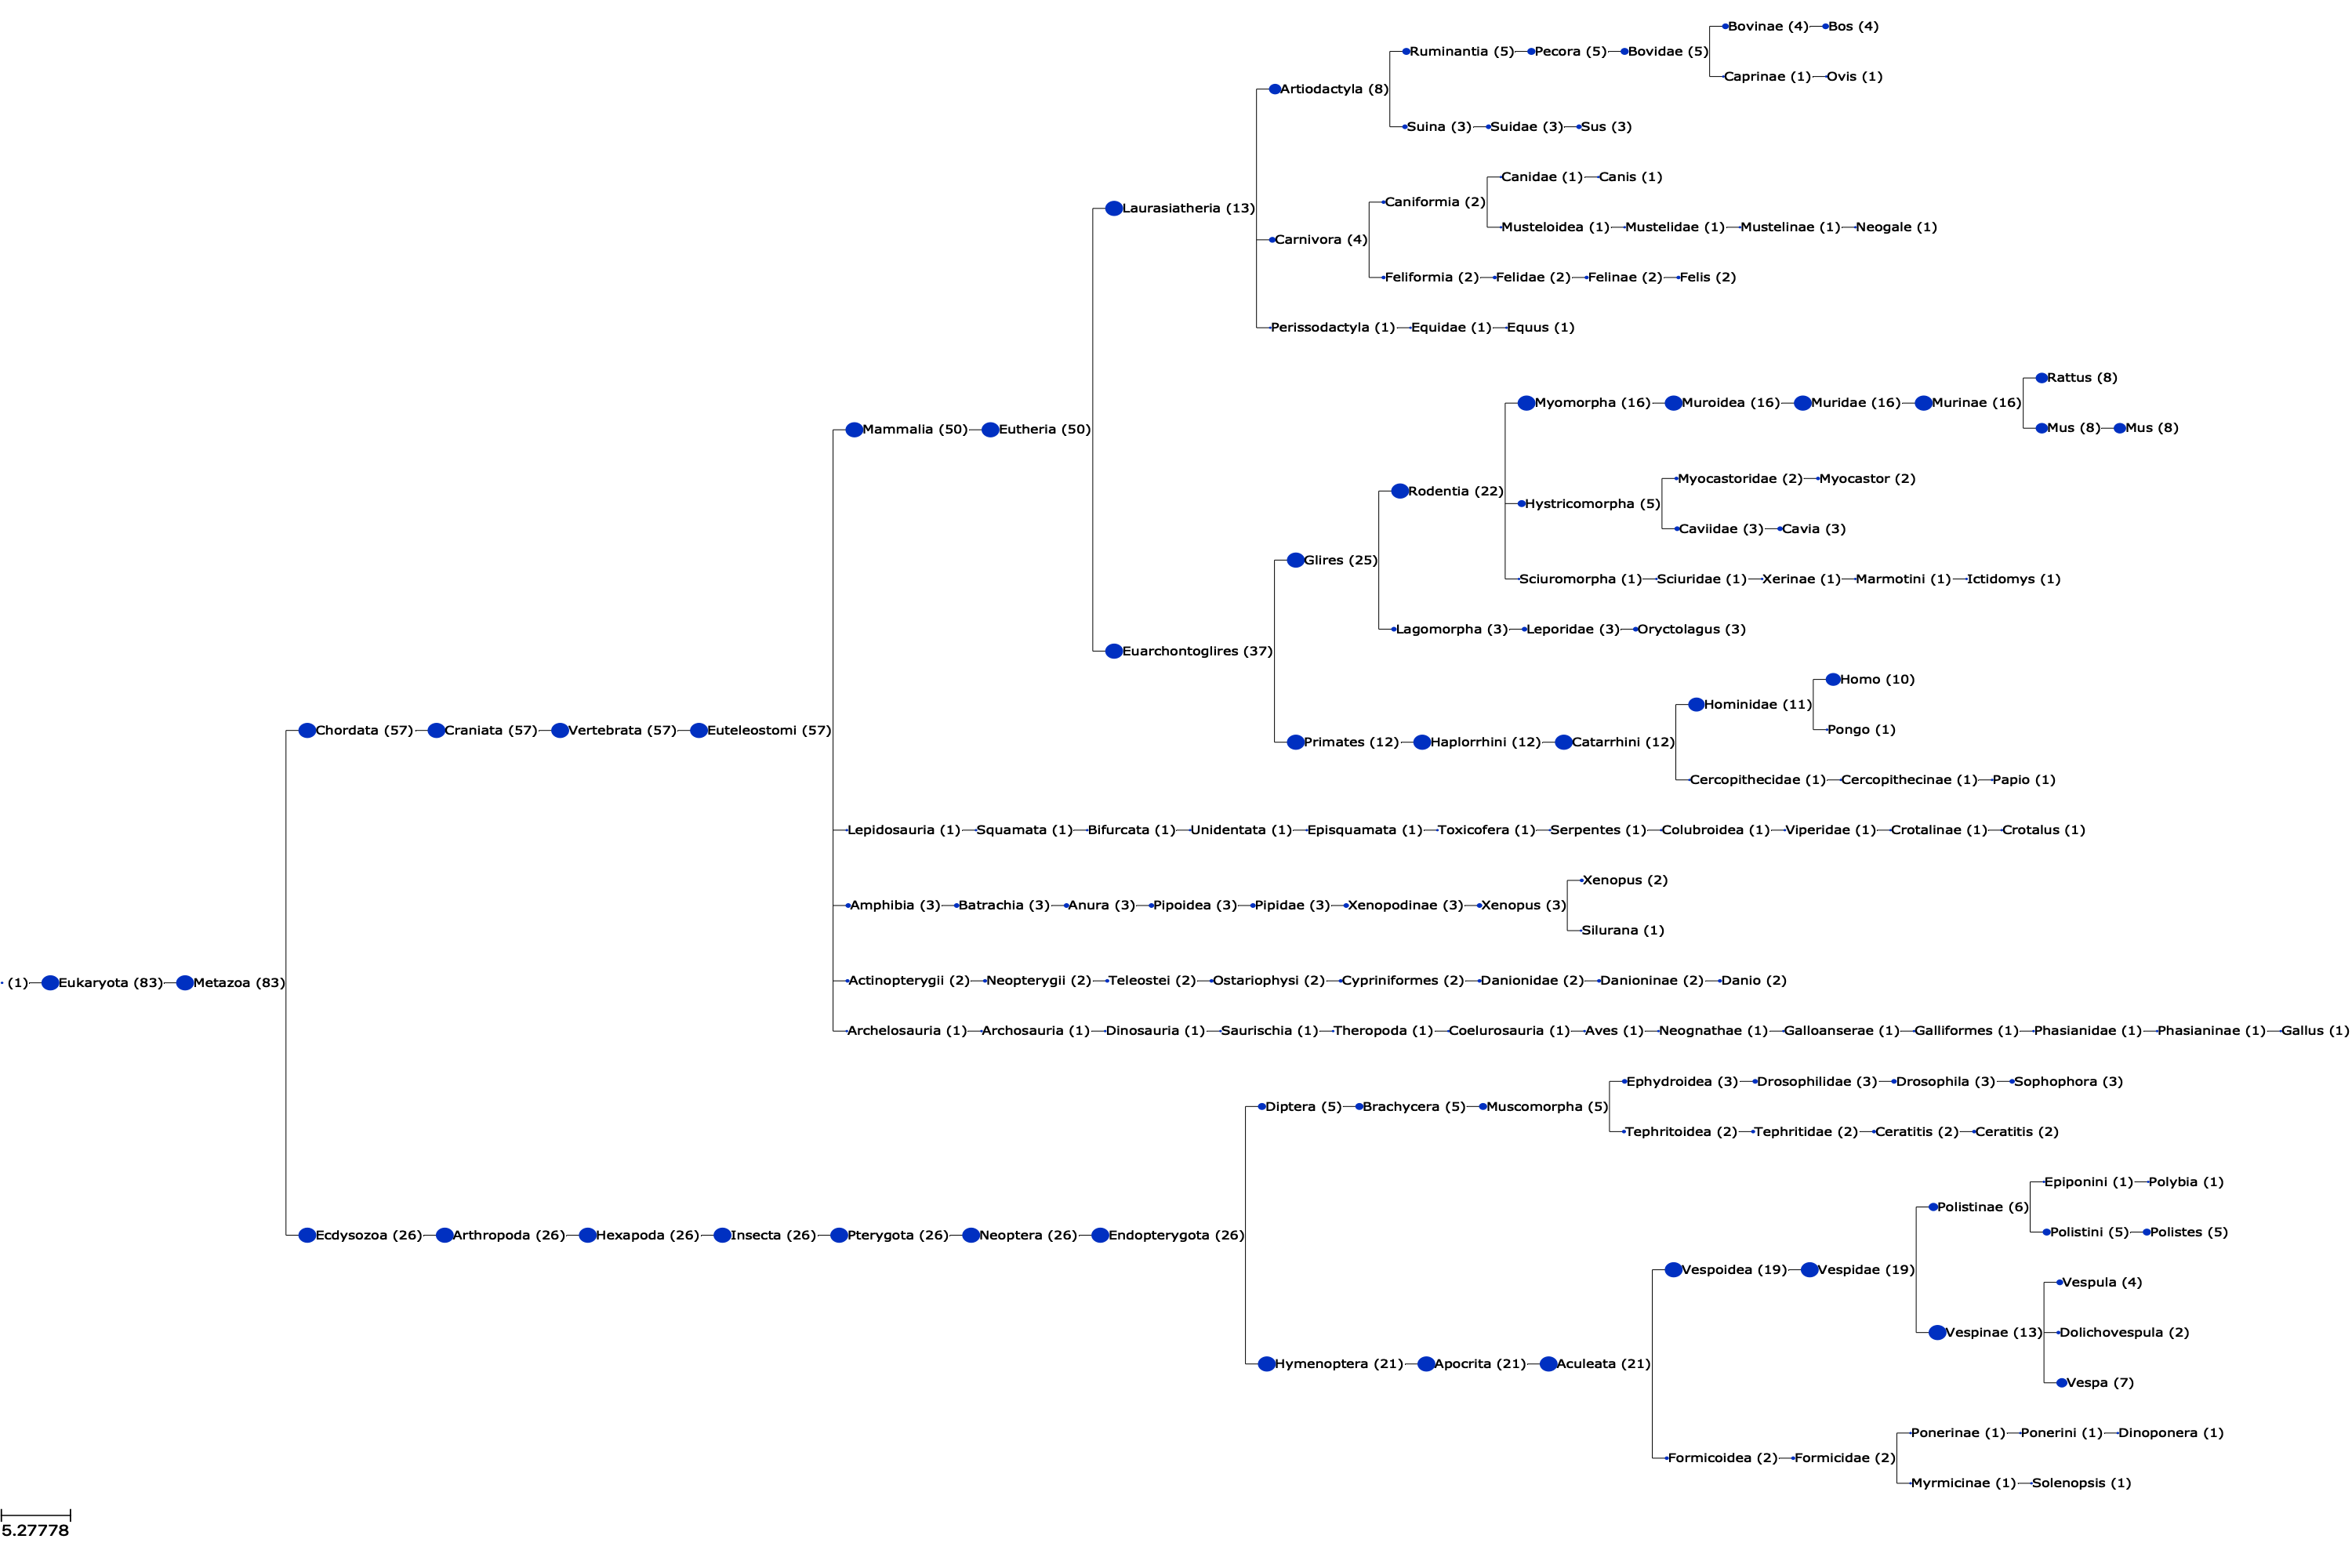
\includegraphics[width=0.9\textwidth]{images/phylogenetic_tree_freq.png}
    \caption{Phylogenetic tree illustrating taxonomic relationships among family sequences. Node sizes reflect relative abundance, highlighting a dominant presence in mammals.}
    \label{fig:phylo-tree}
\end{figure*}
